\section{Heur\'istica de b\'usqueda local}

Volviendo al ejemplo anterior para mostrar que el algoritmo goloso puede ser arbitrariamente malo, podemos observar que una mala soluci\'on del algoritmo goloso puede ``arreglarse'' con relativamente bajo costo.
Partiendo de la soluci\'on a la instancia ``ciclo + estrella de tama\~no $5$'' del algoritmo goloso, basta con mover el nodo que se encuentra compartiendo una partici\'on con el nodo del centro de la estrella. 
Esto puede conseguirse simplemente revisando todos los nodos nuevamente y viendo si se mejora la soluci\'on moviendolos a otra partici\'on.

\begin{figure}[H]
        \centering
        \begin{subfigure}[b]{0.7\textwidth}
                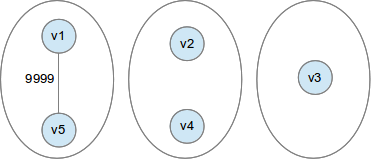
\includegraphics[width=\textwidth]{ej4/local_graph_star+cicle_partition_example1.png}
                \caption{Soluci\'on obtenida mediante el algoritmo goloso, $\omega(S) = 9999$.}
                \label{fig:local_fig_1}
        \end{subfigure}%
         \qquad
         \qquad
         \qquad
         \qquad
         \qquad
         %add desired spacing between images, e. g. ~, \quad, \qquad, \hfill etc.
          %(or a blank line to force the subfigure onto a new line)
        \begin{subfigure}[b]{0.7\textwidth}
                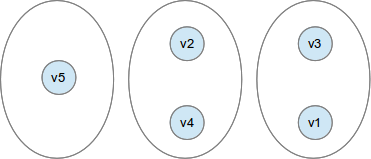
\includegraphics[width=\textwidth]{ej4/local_graph_star+cicle_partition_example2.png}
                \caption{Soluci\'on \'optima del problema, $\omega(S) = 0$.}
                \label{fig:local_fig_2}
        \end{subfigure}
        \caption{Comparaci\'on entre la soluci\'on del algoritmo goloso y la \'optima del problema.}
        \label{greedy_exact_algorithm_comparison}
\end{figure}

Cualquier soluci\'on del algoritmo goloso que se obtenga de una instancia que contenga una componente con la pinta ``ciclo + estrella de tama\~no $n$'' puede ``arreglarse'' de esta forma. Notemos
que como peor caso una soluci\'on de esta instancia tendra varios nodos del ciclo en la misma partici\'on que los del centro de la estrella, luego esa soluci\'on puede mejorarse por otra que mueva cualquiera de esos
nodos a otra partici\'on donde se encuentren otros nodos del ciclo. Esta idea puede generalizarse para dar \'origen a nuestra heur\'istica de busqueda local, tomando una soluci\'on cualquiera (en nuestro caso
generada a partir del goloso) y definiendo como vecindad de esa soluci\'on todas las soluci\'on resultantes de mover un nodo de una partici\'on a otra.\\
Tiene sentido preguntarse si sera cierto que toda soluci\'on puede mejorarse de esta manera. Notemos que si esto fuera cierto y cualquier soluci\'on pudiera mejorarse de esta forma, podr\'ia alcanzarse la soluci\'on
\'optima desde cualquier soluci\'on en tiempo polinomial simplemente realizando sucesivas busquedas locales. El problema radica en que no toda soluci\'on puede ``arreglarse'' moviendo un \'unico nodo de una partici\'on
a otra.\\\

Observemos el siguiente ejemplo:

\begin{figure}[H]
  \centering
  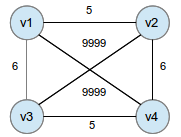
\includegraphics[width=0.4\textwidth]{ej4/local_graph_star+cicle_example1.png}
  \caption{Instancia de un problema 2-PMP.}
\end{figure}
  
\begin{figure}[H]
        \centering
        \begin{subfigure}[b]{0.6\textwidth}
                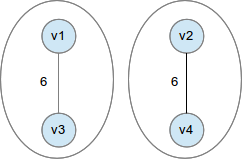
\includegraphics[width=\textwidth]{ej4/local_graph_star+cicle_partition_example3.png}
                \caption{Soluci\'on obtenida mediante el algoritmo goloso, $\omega(S) = 12$.}
                \label{fig:greedy_fig_3}
        \end{subfigure}%
         \qquad
         \qquad
         \qquad
         \qquad
         \qquad
         %add desired spacing between images, e. g. ~, \quad, \qquad, \hfill etc.
          %(or a blank line to force the subfigure onto a new line)
        \begin{subfigure}[b]{0.6\textwidth}
                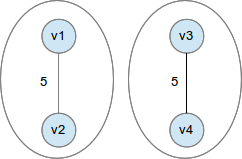
\includegraphics[width=\textwidth]{ej4/local_graph_star+cicle_partition_example4.png}
                \caption{Soluci\'on \'optima del problema, $\omega(S) = 10$.}
                \label{fig:greedy_fig_4}
        \end{subfigure}
        \caption{Ejecuci\'on del algoritmo greedy paso por paso.}
        \label{greedy_algorith_example2}
\end{figure}

En este ejemplo en particular, esta claro que todas las soluciones vecinas a la soluci\'on propuesta por el goloso son se alejan bastante del \'optimo (de hecho arbitrariamente seg\'un el peso que asignemos
a las aristas diagonales). Vamos a exhibir una familia de grafos donde la vecindad de la soluci\'on obtenida por el algoritmo goloso, no puede mejorarse moviendo un \'unico nodo a otra partici\'on y esta soluci\'on puede alejarse del \'optimo
tanto como queramos. \\\

\begin{figure}[H]
  \centering
  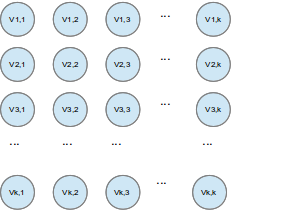
\includegraphics[width=0.4\textwidth]{ej4/local_graph_star+cicle_example2.png}
  \caption{Instancia de un problema 2-PMP.}
\end{figure}

Pensando la siguiente familia de grafos como una matriz, supongamos que existe una arista que une cada par de nodos $(v_{i,i}, v_{i, i+1})$ horizontalmente de forma tal que el \'optimo se alcanza agrupando los nodos horizontalmente en k particiones.
Ademas existe una arista entre todos par de nodos que no pertenezcan a la misma partici\'on (columna) ni a la misma fila y estas aristas son m\'as pesadas que la suma de todas las aristas que existan entre nodos de una misma columna.
De esta forma, siguiendo un \'orden lexicografico que recorre por filas y luego por columnas los resultados tendr\'ian la siguiente pinta:

\begin{figure}[H]
        \centering
        \begin{subfigure}[b]{0.6\textwidth}
                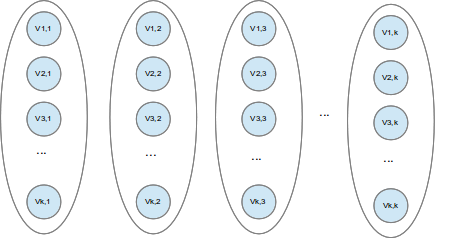
\includegraphics[width=\textwidth]{ej4/local_graph_star+cicle_partition_example5.png}
                \caption{Soluci\'on obtenida mediante el algoritmo goloso, $\omega(S) = L_{1}$.}
                \label{fig:greedy_fig_3}
        \end{subfigure}%
         \qquad
         \qquad
         \qquad
         \qquad
         \qquad
         %add desired spacing between images, e. g. ~, \quad, \qquad, \hfill etc.
          %(or a blank line to force the subfigure onto a new line)
        \begin{subfigure}[b]{0.3\textwidth}
                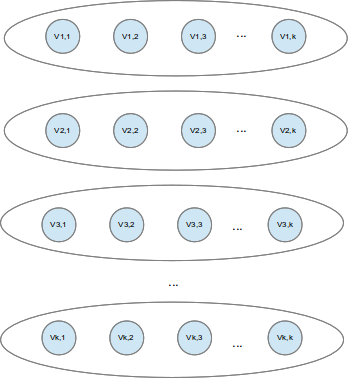
\includegraphics[width=\textwidth]{ej4/local_graph_star+cicle_partition_example6.png}
                \caption{Soluci\'on \'optima del problema, $\omega(S) = L_{2}$.}
                \label{fig:greedy_fig_4}
        \end{subfigure}
        \caption{Ejecuci\'on del algoritmo greedy paso por paso.}
        \label{greedy_algorith_example2}
\end{figure}

Como existe una arista entre todo nodo que no pertenezca a la misma fila o la misma columna m\'as pesada que la suma de todas las aristas de la misma columna, nunca puede mejorarse la soluci\'on moviendo un
nodo de una partici\'on a otra, ya que el peso aumentaria por las aristas que conectan al nodo con el resto de la partici\'on. Sin embargo, las aristas horizontales entre todo par de nodos son las menos pesadas
por lo que no se alcanza el optimo. Esta diferencia ademas puede ser tan mala como queramos.
 

\subsection{Algoritmo}

\subsubsection{An\'alisis de complejidad}

\subsection{Experimentaci\'on}
